\documentclass[landscape]{article}
\usepackage[a4paper,margin=1.4cm]{geometry}
\usepackage[utf8]{inputenc}
\usepackage[T1]{fontenc}
\usepackage{multicol}
\usepackage{lipsum}
\usepackage{amsmath}
\usepackage{amsfonts}
\usepackage{tikz}
\usepackage{xcolor}

\usepackage{graphicx}
\graphicspath{ {./images/} }

\setlength{\columnsep}{1cm}
\renewcommand{\columnseprulecolor}{\normalcolor}
% set \paragraph vertical spacing
\makeatletter
\renewcommand{\paragraph}{\@startsection{paragraph}{4}{\z@}%
                                    {3ex}%
                                    {-0.75em}%
                                    {\normalfont\normalsize\bfseries}}
\makeatother
% reduce space before \subparagraph
\makeatletter
\renewcommand{\subparagraph}{\@startsection{subparagraph}{5}{\z@}%
                                       {2ex}%
                                       {-0.75em}%
                                       {\normalfont\normalsize\bfseries\hspace{1.25em}}}% Add \hspace{1.25em} for 1 level of indent
\makeatother
% add vertical space before \minipage and rename environment to \minipage
\let\oldminipage\minipage
\let\endoldminipage\endminipage
\renewenvironment{minipage}{\vspace{0.5em}\begin{oldminipage}{0.925\linewidth}}{\end{oldminipage}}

% Custom command for horizontal separator
\newcommand{\sep}{\noindent\rule{\linewidth}{0.4pt}}

% remove page numbering
\pagenumbering{gobble}

\begin{document}
\begin{multicols*}{3}
       \footnotesize % Change the font size here if needed

       \section*{MAT2 - Mathématiques\\ \small{Leonard Cseres - Mars 2024}}
       \paragraph{Angles}\mbox{}\\
       \begin{tabular}{p{4em}|c|c|c|c|c|c|c|c}
              $\theta$ & $0$ & $\frac{\pi}{6}$      & $\frac{\pi}{4}$      & $\frac{\pi}{3}$      & $\frac{\pi}{2}$ & $\pi$ & $\frac{3\pi}{2}$ & $2\pi$ \\
              \hline
              $\sin$   & $0$ & $\frac{1}{2}$        & $\frac{\sqrt{2}}{2}$ & $\frac{\sqrt{3}}{2}$ & $1$             & $0$   & $-1$             & $0$    \\
              $\cos$   & $1$ & $\frac{\sqrt{3}}{2}$ & $\frac{\sqrt{2}}{2}$ & $\frac{1}{2}$        & $0$             & $-1$  & $0$              & $1$    \\
              $\tan$   & $0$ & $\frac{\sqrt{3}}{3}$ & $1$                  & $\sqrt{3}$           & $\infty$        & $0$   & $\infty$         & $0$    \\
       \end{tabular}\vspace{0.5em}\\
       \begin{tabular}{p{4em}|c|c|c|c|c}
              $x$          & $0$ & $\frac{1}{\sqrt{3}}$ & $1$             & $\sqrt{3}$      & $\infty$        \\
              \hline
              $\arctan(x)$ & $0$ & $\frac{\pi}{6}$      & $\frac{\pi}{4}$ & $\frac{\pi}{3}$ & $\frac{\pi}{2}$ \\
       \end{tabular}

       \section*{Calcul différentiel}
       \paragraph{Valeur moyenne} $f(c) = \frac{1}{b-a} \int_{a}^{b} f(x)dx, \quad a, b \in \mathbb{R}$
       \paragraph{Primitives}
       \begin{flalign*}
               & \int f(x)^a \cdot f'(x)dx         = \frac{1}{a+1}f(x)^{a+1} + C, \quad C \in \mathbb{R} & \\
               & \int \frac{f'(x)}{1 + (f(x))^2}dx = \arctan(f(x)) + C, \quad C \in \mathbb{R}           &
       \end{flalign*}
       \paragraph{Aucune racine réelle}
       \begin{flalign*}
               & \int \frac{\alpha(2ax+b)}{ax^2+b x+c}dx = \alpha\ln\left|a x^2+b x+c\right| + C, \quad C \in \mathbb{R}                                   & \\
               & \int \frac{\beta}{a x^2+b x+c}dx = \frac{2\beta}{\sqrt{4 a c-b^2}} \arctan\left(\frac{2ax+b}{\sqrt{4ac-b^2}}\right) + C, C \in \mathbb{R} &
       \end{flalign*}

       \paragraph{Intégrales impropres} Si la limite existe, l'intégrale est \textit{convergente}, sinon elle est \textit{divergente}.


       \subparagraph{Type I} Soit $f$ \textit{continue} sur l'intervalle et possède une asymptote horizontale en $+\infty$ ou $-\infty$, alors
       \begin{flalign*}
               & \int_{a}^{+\infty} f(x)dx = \lim_{t \to +\infty} \int_{a}^{t} f(x)dx, \quad a \in \mathbb{R}                    & \\
               & \int_{-\infty}^{b} f(x)dx = \lim_{t \to -\infty} \int_{t}^{b} f(x)dx, \quad b \in \mathbb{R}                    & \\
               & \int_{-\infty}^{+\infty} f(x)dx = \int_{-\infty}^{a} f(x)dx + \int_{a}^{+\infty} f(x)dx, \quad a \in \mathbb{R} &
       \end{flalign*}
       \subparagraph{Type II} Soit $f$ \textit{continue} sur l'intervalle et possède une asymptote verticale en $c \in \ ]a, b[$, alors
       \begin{flalign*}
               & \int_{a}^{b} f(x)dx = \lim_{t \to b_{-}} \int_{a}^{t} f(x)dx, \quad a \in \mathbb{R}  & \\
               & \int_{a}^{b} f(x)dx = \lim_{t \to a_{+}} \int_{t}^{b} f(x)dx, \quad b \in \mathbb{R}  & \\
               & \int_{a}^{b} f(x)dx = \int_{a}^{c} f(x)dx + \int_{c}^{b} f(x)dx, \quad c \in \ ]a, b[ &
       \end{flalign*}

       \columnbreak

       \section*{Géométrie}
       \paragraph{Espace $\mathbb{R}^3$}
       \subparagraph{Équation de la droite}
       \begin{itemize}
              \item \textbf{Cartésienne} $\begin{cases} A_1x_1 + A_2x_2 + A_3x_3 + A_4 = 0 \\
                                  B_1x_1 + B_2x_2 + B_3x_3 + B_4 = 0\end{cases}$
              \item \textbf{Paramétrique} $\vec{x} = \vec{a} + \lambda \vec{u}$, $\quad\lambda \in \mathbb{R}$
       \end{itemize}
       \subparagraph{Équation de $\pi$}
       \begin{itemize}
              \item \textbf{Cartésienne} $A_1x_1 + A_2x_2 + A_3x_3 + A_4 = 0$
              \item \textbf{Paramétrique} $\vec{x} = \vec{a} + \lambda \vec{u} + \mu \vec{v}$, $\quad\lambda, \mu \in \mathbb{R}$
       \end{itemize}
       \paragraph{Tétraèdre}\mbox{}\\
       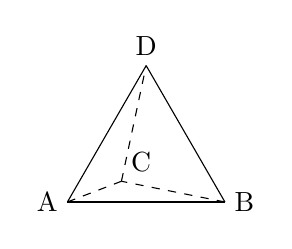
\begin{tikzpicture}
              \coordinate (A) at (0,0,0);
              \coordinate (B) at (2,0,0);
              \coordinate (C) at (1,{sqrt(3)/3},{sqrt(6)/3});
              \coordinate (D) at (1,{sqrt(3)},0);
              \draw (A) -- (B);
              \draw (A) -- (D);
              \draw (B) -- (D);
              \draw[dashed] (A) -- (C);
              \draw[dashed] (B) -- (C);
              \draw[dashed] (C) -- (D);
              \node[left] at (A) {A};
              \node[right] at (B) {B};
              \node[above right] at (C) {C};
              \node[above] at (D) {D};
       \end{tikzpicture}\\
       \hspace*{0.75em}$V = \frac{1}{6}\left|\det(\vec{a}, \vec{b}, \vec{c})\right|$

       \color{gray}
       \section*{Combinatoire}
       \scalebox{0.905}{
              \begin{tabular}{l|c|c|c}
                     \textbf{Nom}          & \textbf{Formule}                      & \textbf{Répétition} & \textbf{Ordre} \\
                     \hline
                     \hline
                     Permutation           & $P_n = n!$                            & Non                 & Oui            \\
                     \hline
                     Arrangement           & $A_k^n = \frac{n!}{(n-k)!}$           & Non                 & Oui            \\
                     Arrangement avec rép. & $\overline{A}_k^n = n^k$              & Oui                 & Oui            \\
                     \hline
                     Combinaison           & $C_k^n = \binom{n}{k}$                & Non                 & Non            \\
                     Combinaison avec rép. & $\overline{C}_k^n = \binom{n+k-1}{k}$ & Oui                 & Non            \\
              \end{tabular}
       }
       \color{black}

       \paragraph{Partitions} Le nombre de façons de diviser $n$ éléments en $k$ groupes de tailles $n_1, n_2, \ldots, n_k$ est donné par $\overline{P}(n_1, n_2, \ldots, n_k) = \frac{n!}{n_1!n_2!\ldots n_k!}$

       \section*{Moindres carrés}
       $\textbf{A}\vec{x} = \vec{b}$, $\quad\textbf{A}^T\textbf{A}\vec{x} = \textbf{A}^T\vec{b}$, $\quad\vec{x}^* = (\textbf{A}^T\textbf{A})^{-1}\textbf{A}^T\vec{b}$\vspace*{0.5em}

       \par Le système $\textbf{A}\vec{x} = \vec{b}$ est inconsistant si et seulement si la matrice augmentée $[\textbf{A}|\vec{b}]$ possède un \textbf{1 directeur en dernière colonne}.

       \section*{Dérivées et primitives}
       \paragraph{Dérivées usuelles}
       \begin{flalign*}
               & (f(g(x)))' = f'(g(x)) \cdot g'(x)      & \\
               & (f^{-1}(x))' = \frac{1}{f'(f^{-1}(x))} & \\
               & \arccos'(x) = -\frac{1}{\sqrt{1-x^2}}  & \\
               & \arcsin'(x) = \frac{1}{\sqrt{1-x^2}}   & \\
               & \arctan'(x) = \frac{1}{1+x^2}          &
       \end{flalign*}

       \paragraph{Primitives usuelles}
       \begin{flalign*}
               & \int \frac{1}{x}dx = \ln|x| + C, \quad C \in \mathbb{R}         & \\
               & \int \tan(x) = -\ln|\cos(x)| + C, \quad C \in \mathbb{R}        & \\
               & \int \frac{1}{1+x^2}dx = \arctan(x) + C, \quad C \in \mathbb{R} & \\
       \end{flalign*}


\end{multicols*}
\end{document}
